\documentclass[12pt]{article}

\usepackage{amsmath}
\usepackage{physics}
\usepackage{hyperref}
\usepackage{siunitx}
\DeclareSIUnit\poundforce{lbf}
\DeclareSIUnit\foot{ft}
\usepackage{graphicx}
\usepackage[super]{nth}

% Aspect ratio symbol for wings
\newcommand{\ar}{A\mkern-6mu R}

\usepackage[style=ieee, backend=bibtex]{biblatex}
\renewcommand{\bibfont}{\small}
\addbibresource{references_for_compressible_aero.bib}


\title{Modeling Transonic Aerodynamics in Geometric Programs}

\author{Matthew Vernacchia\\
Department of Aeronautics and Astronautics, MIT}

\date{\today}

\begin{document}
\maketitle
This document discusses techniques and challenges for modeling the aerodynamics of transonic aircraft within the geometric programming optimization framework.

This work is done to support an exploration of the small and fast aircraft design space. It is part of the Firefly project, sponsored by BAE Systems and MIT Lincoln Laboratories.


\section{Fuselage}
\subsection{Fuselage Drag}
Fleeman \cite{Fleeman2012} presents the following formulas for the transonic drag of a cylindrical fuselage with a sharp (ogive?) nose. He breaks the drag coefficient into three components: friction, drag, base drag and wave drag:

\begin{equation}
C_{D0, fuse} = C_{D0, fric} + C_{D0, base} + C_{D0, wave}
\end{equation}

This expression can be written as a GP-compatible inequality constrain:
\begin{equation}
C_{D0, fuse} \geq C_{D0, fric} + C_{D0, base} + C_{D0, wave}
\end{equation}
The optimization "pressure" to minimize drag should keep this contraint tight.

\subsubsection{Friction Drag}
The friction drag is correlated with Mach number $M$, the fuselage length $l$, the fuselage diameter $d$, and the dynamic pressure $q$. Fleeman based this correlation on the work of Jerger \cite{Jerger1960}.

\begin{equation}
\label{eq:c_d_fric}
C_{D0, fric} = (\SI{0.053}{\poundforce^{0.2} \foot^{-0.2}}) (l/d) \left( \frac{M}{q l} \right)^{0.2}
\end{equation}

I have inferred the units on the leading parameter in order to make $C_{D}$ dimensionless based on the units for $q$ and $l$ used in Fleeman figure 2.7. the right-hand side of Equation \ref{eq:c_d_fric} is a positive monomial in $l, d, M, q$; thus the equation is GP-compatible as an equality constraint.


\subsubsection{Base and Wave Drag}
Fleeman suggests the following approximate correlation for the base drag
\begin{equation}
C_{D0, base} = 
  \begin{cases}
    0.12 + 0.13 M^2 & M < 1 \\
    \frac{0.25}{M} & M \geq 1 \
  \end{cases}
\end{equation}

This piecewise function is $C^0$ continuous, but not smooth. It is not GP-compatible.

Fleeman suggests approximating the wave drag as:
\begin{equation}
C_{D0, wave} = 
  \begin{cases}
    0 & M < 1 \\
    (1.586 + 1.834/M^2) \left( \arctan(\frac{0.5}{(l_N/d)})\right)^{1.69} & M \geq 1 \
  \end{cases}
\end{equation}

where $(l_N/d)$ is the fineness ratio of the nose. This function is discontinuous in Mach number at $M = 1$. It is not GP-compatible.

\subsubsection{Comparison with Experimental Data}

Similar $C_{D0} \approx 0.2$ at subsonic.
Similar rapid increase approaching Mach 1.
Fleeman predicts sharp peak of $C_{D0} = 0.5$
Hoerner data shows rounded peak of $C_{D0} = 0.4$ to $0.45$ from $M = 1$ to $1.5$.

\begin{figure}[hbt!]
    \centering
    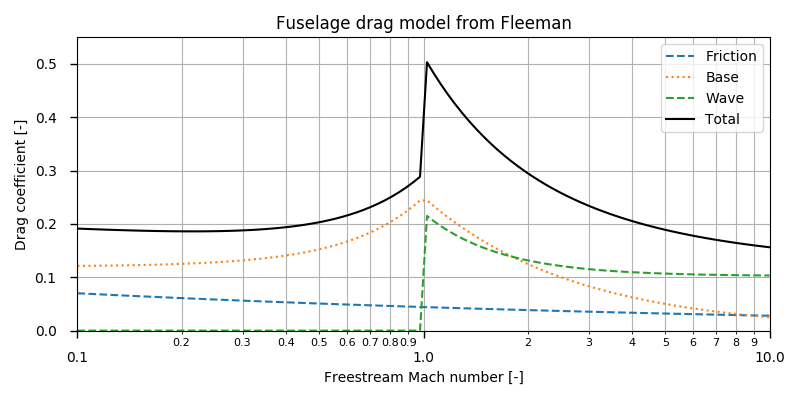
\includegraphics[width=1\textwidth]{figures/fleeman_fuselage_drag_model}
    \caption{\label{fig:fleeman_fuselage_drag_model} Fleeman's fuselage drag model. Assuming nose fineness ratio of $2.5$, body length of \SI{0.5}{\meter}, body fineness ratio of $5$, and static pressure of \SI{30}{\kilo\pascal}.}
\end{figure}

\begin{figure}[hbt!]
    \centering
    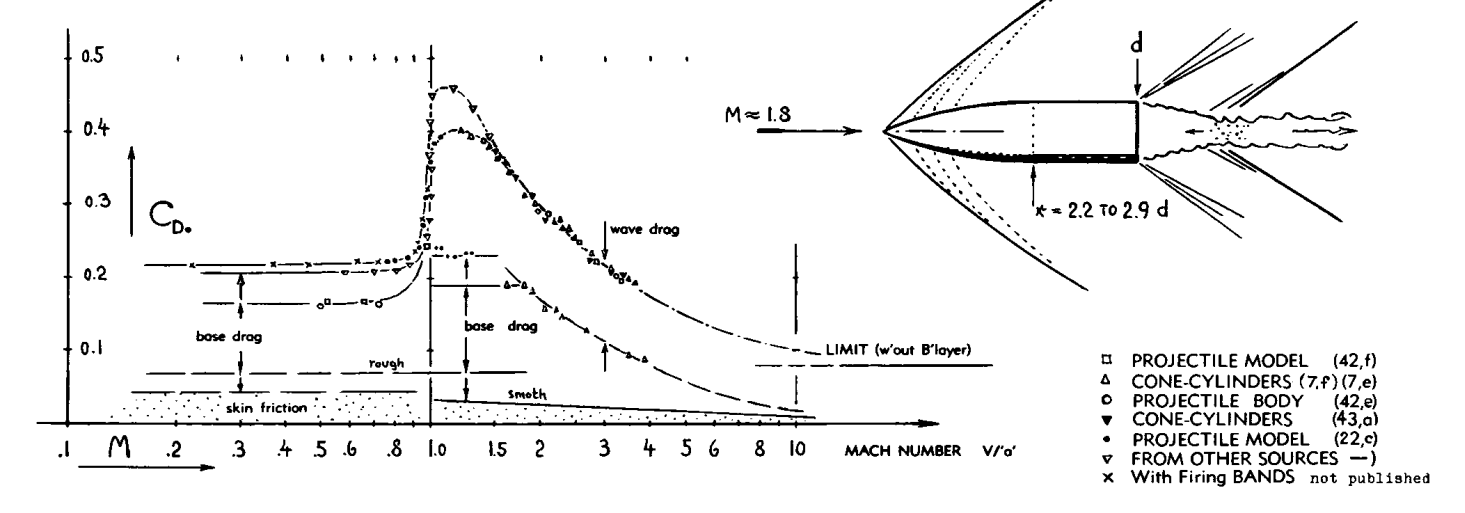
\includegraphics[width=1\textwidth]{figures/hoerner_fig_16_30}
    \caption{\label{fig:hoerner_fig_16_30} Hoerner's compilation of drag data on smooth projectile bodies. These drag coefficients should be comparable to Fleeman's model.}
\end{figure}


\subsubsection{Approaches to use with Geometric programming}
The transonic drag model given in \cite{Fleeman2012} is not, as given, compatible with geometric programming. This is because the drag coefficient vs. Mach number function, $C_D(M)$, is discontinuous and non-monotonic. Therefore, it cannot be represented by a monomial equality constraint. I also suspect that it cannot be represented by a set of posinomial inequality constraints, but I do not know how to prove that.

I suggest two approaches to sidestep this issue: 1) implement the drag model as an external, non-GP model; or 2) perform separate optimizations for transonic vs. supersonic aircraft.

\paragraph{Non-GP model}
GPKit provides an interface for including external, non-GP compatible models in the optimization, and then solving via successive local GP approximations of the problem.
A example of the interface is provided in the GPKit documentation [\href{https://gpkit.readthedocs.io/en/latest/signomialprogramming.html#sequential-geometric-programs}{link}].

\paragraph{Separate subsonic vs. supersonic optimizations}
Fleeman's drag model is GP-compatible if we restrict it to only the subsonic ($M<1$) or only the supersonic ($M > 1$) regimes \footnote{The wave drag equation contains an arctangent function, which is compatible with GPkit. However, the argument to arctan is small ($\in [0, 1]$), so we can use the $\arctan(x) \approx x$ approximation without too much error.}. Thus, we can sidestep this issue if we are willing to constrain the optimization to only run on subsonic or only run on supersonic vehicles.

Pros:
\begin{itemize}
    \item Easier to implement than non-GP model option.
    \item Maintains GP fast-solve and global optimality guarantees, unlike non-GP model option.
    \item Subsonic vs. supersonic aircraft may be quite different in their design and missions, so maybe it's not a big deal to have them as separate optimizations.
    \item If we really do want to assess the subsonic vs. supersonic tradeoff for a particular mission, we can solve for the optimal subsonic aircraft, separately solve for the optimal supersonic aircraft, then compare the two.
\end{itemize}

Cons:
\begin{itemize}
    \item Less general/elegant than having a single model for all Mach numbers.
\end{itemize}


\section{Wing}
\subsection{Lift}
We wish to model the lift of a finite, swept wing in compressible flow.
Several models have been proposed for this situation.
They all share the following variables:

\begin{description}
    \item[$C_{L\alpha}$] The lift slope $\pdv{C_L}{\alpha}$ of the 3D wing.
    \item[$c_{l, \alpha, inc}$] The lift slope $\pdv{c_l}{\alpha}$ of the 2D airfoil in incompressible flow, or $c_{l, \alpha, M}$, the lift slope curve of the 2D airfoil at the given Mach number.
    \item[$\Lambda$] The sweep angle of the wing. Note that the sweep angle is defined differently in different sources, e.g. along the leading edge, half-chord point, or maximum thickness chord point.
    \item[$\ar$] The aspect ratio of the wing.
    \item[$M_{\infty}$] The freestream Mach number.
\end{description}

We want a GP-compatible constraint relation between these variables. The ``optimization pressure'' will be to maximize $C_{L\alpha}$, so we want $C_{L\alpha}$ to be bounded from above by the constrain. A possible constraint form would be:

\begin{equation}
\frac{1}{C_{L\alpha}} = g(c_{l\alpha}, \Lambda, \ar, M_\infty)
\end{equation}

where $g$ is a posynomial.

\subsubsection{Comparison of Lift Models}

Unfortunately, different sources give different models relating these variables. Some of these models are summarized below:

\paragraph{DATCOM Model}
Raymer \cite{Raymer2012} suggests the following model from the UASF DATCOM:

\begin{equation}
C_{L\alpha} = \frac{2 \pi \ar}{2 + \sqrt{4 + \frac{4 \ar^2 \pi^2}{c_{l\alpha, M}^2} \left( 1 + \frac{\tan^2(\Lambda)}{\beta^2} \right)}}
\end{equation}

This model is ``semi-empirical,'' and Raymer claims it is ``reasonable accurate almost to Mach 1 for a swept wing'' \cite{Raymer2012}. 
TODO Is $\beta$ based on $M_\infty$ or $M_\perp$??
I think this can be written in a GP compatible form (TODO see paper notes).

\paragraph{Anderson's Model}
Anderson suggests the following model (Eq. 2.22 in \cite{Anderson1999}):

\begin{equation}
C_{L,\alpha} = \frac{c_{l\alpha, inc} \cos\Lambda}{
\sqrt{\beta^2 + \left( \frac{c_{l\alpha, inc} \cos\Lambda}{\pi \ar} \right)^2}
+ \frac{c_{l\alpha, inc} \cos\Lambda}{\pi \ar}}
\end{equation}

Anderson derives this equation by taking his incompressible swept wing equation (Eq. 2.19 in \cite{Anderson1999}) and substituting $c_{l\alpha, inc}/\beta$ for $c_{l\alpha}$. However, Drela's explanation of the Prandtl-Glauer transform (Ch. 8.6 in \cite{Drela2014}) suggests that we should also substitute $\beta \ar$ for $\ar$ and a complicated expression (Eq. 8.100 in \cite{Drela2014}) for $\cos(\Lambda)$.

This model will be more difficult to put into a GP-compatible form, as it contains the cosine of a decision variable. The Taylor expansion for cosine about zero is not a posynomial (negative coefficients).

\paragraph{Drela's Model}
Drela's book \cite{Drela2014} does not provide a formula for a swept, finite wing. it does provide separate formulas for a finite rectangular wing and a infinite swept wing:

\begin{equation}
\Lambda = 0: C_{L\alpha} = \frac{c_{l\alpha, inc}}{\beta + \frac{c_{l\alpha, inc}}{\pi \ar}}
\end{equation}

\begin{equation}
\ar \rightarrow \infty : C_{L\alpha} = \frac{c_{l\alpha, inc} \cos\Lambda}{
    \sqrt{\beta^2 \cos^2\Lambda + \sin^2\Lambda}}
\end{equation}
where $\beta = \sqrt{1 - M_\infty^2}$

This model will be more difficult to put into a GP-compatible form, as it contains $\cos, \cos^2$ and $\sin^2$ of a decision variable. The Taylor expansion for these functions about zero are not posynomials (negative coefficients).

Drela provides a clear derivation of these equations via the Prandtl-Glauert transformation and lifting-line theory. 


\paragraph{Comparing the DATCOM model to Drela's Prandtl-Glauert-based model}
Below are several plots comparing the DATCOM model to Drela's Model. Because Drela's model is derived via the Prandtl-Glauert transformation, we should expect it to diverge to unrealistically high $C_{L\alpha}$ as $M \rightarrow 1$. Because Drela's model is derived from lifting line theory, we should expect it to be less accurate at low $\ar$, and more accurate at high $\ar$.
Drela's model should be exact (?) at the extreme of $M \rightarrow 0, \ar \rightarrow \infty$. Thus, we should expect the DATCOM model to match Drela's model at that extreme.

The plots indicate that the DATCOM model does match/approach Drela's model where the assumptions of Drela's theory are valid (low $M$, high $\ar$). Also, the DATCOM model always predicts lower $C_{L\alpha}$ than Drela's model. This is another point in favor of the DATCOM model, as it is more conservative to use a model which gives lower estimates for lift.

\begin{figure}[hbt!]
    \centering
    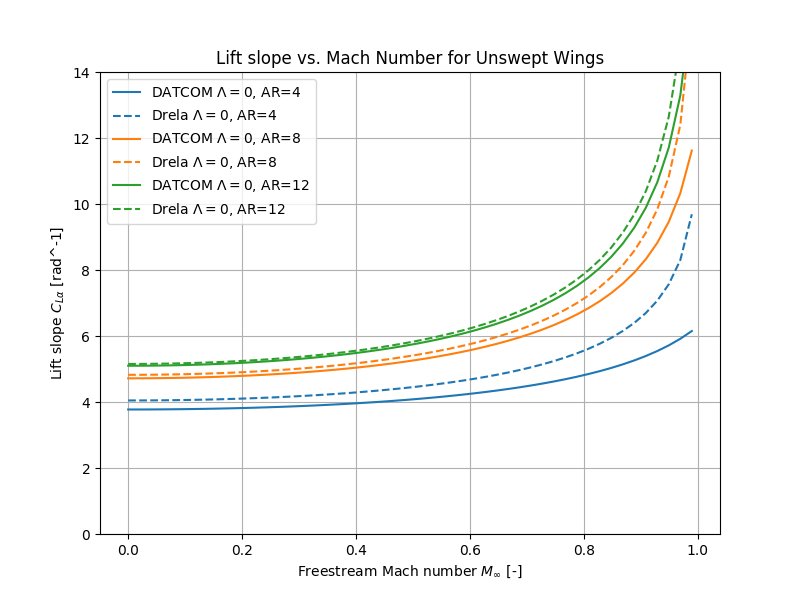
\includegraphics[width=1\textwidth]{figures/wing_lift_model_compare/CLa_vs_mach}
    \caption{\label{fig:wing_model_CLa_vs_mach} Comparison of the DATCOM model and Drela's model vs. Mach number. The DATCOM model matches Drela's model at low $M$, and predicts lower $C_{L\alpha}$ than Drela's model as $M \rightarrow 1$. These are both indications that the DATCOM model is sound.}
\end{figure}

\begin{figure}[hbt!]
    \centering
    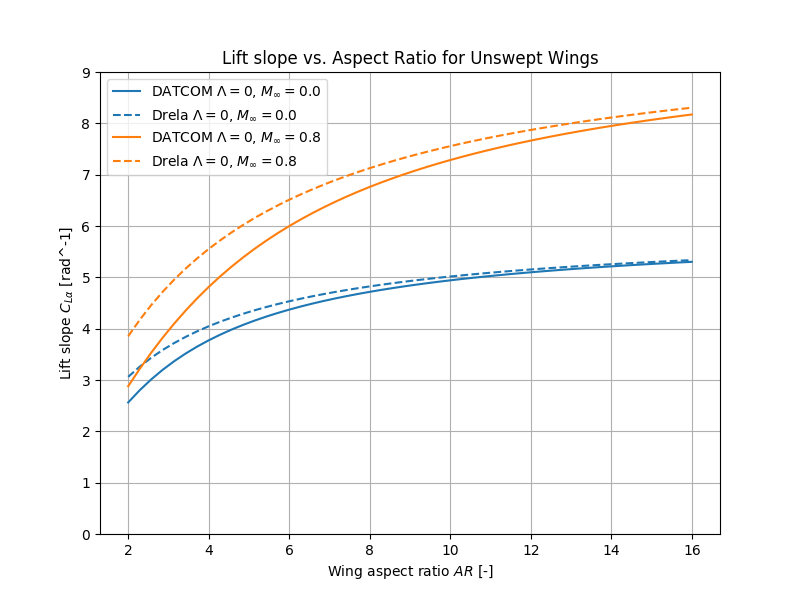
\includegraphics[width=1\textwidth]{figures/wing_lift_model_compare/CLa_vs_aspect}
    \caption{\label{fig:wing_model_CLa_vs_aspect} Comparison of the DATCOM model and Drela's model vs. aspect ratio. The DATCOM model approaches Drela's model at high $\ar$, and predicts lower $C_{L\alpha}$ than Drela's model low $\ar$. These are both indications that the DATCOM model is sound.}
\end{figure}

\begin{figure}[hbt!]
    \centering
    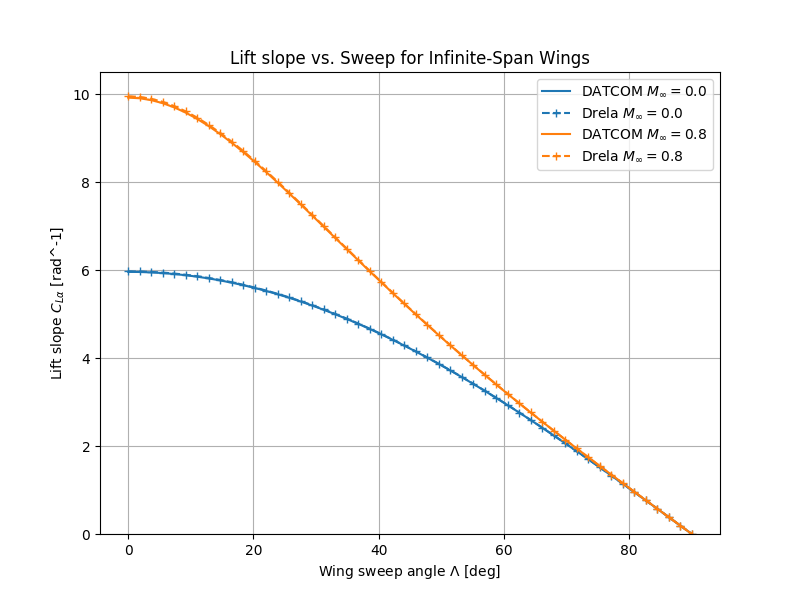
\includegraphics[width=1\textwidth]{figures/wing_lift_model_compare/CLa_vs_sweep}
    \caption{\label{fig:wing_model_CLa_vs_sweep} Comparison of the DATCOM model and Drela's model vs. sweep. The DATCOM model matches Drela's model almost exactly in the limit $\ar \rightarrow \infty$. This is an indication that the DATCOM model is sound.}
\end{figure}


\subsubsection{GP implementation of DATCOM model}
The following plots compare the DATCOM model as given in \cite{Raymer2012} to my GPkit implementation of that model. Figure \ref{fig:wing_model_GP_mach} shows that the models match exactly across a range of Mach numbers at zero sweep. This verifies that the GPkit model has been implemented correctly.

Figure \ref{fig:wing_model_GP_sweep} shows that the GPkit implementation diverges from the DATCOM model as sweep $\Lambda$ increases. This is because of a Taylor series approximation used in the model. The DATCOM model contains a $\tan^2(\Lambda)$ term. This term is not GP compatible, so the GP model approximates $\tan^2(\Lambda)$ with a \nth{12} order Taylor series, which is a GP-compatible posynomial. The Taylor series and $\tan^2(\Lambda)$ are compared in the bottom part of Figure \ref{fig:wing_model_GP_sweep}. The model is usably accurate up to a sweep angle of about \SI{70}{\degree} (grey vertical line in Figure \ref{fig:wing_model_GP_sweep}).

\begin{figure}[hbt!]
    \centering
    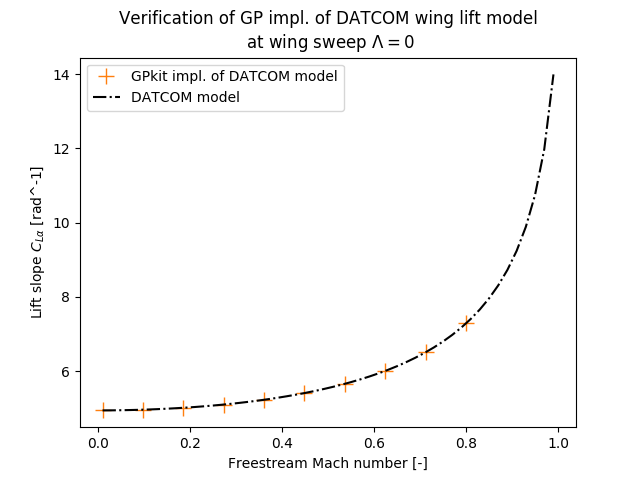
\includegraphics[width=0.8\textwidth]{figures/wing_lift_model_compare/GP_mach}
    \caption{\label{fig:wing_model_GP_mach} Comparison of $C_{L\alpha}$ vs. $M_\infty$ predictions for the DATCOM model (as given in \cite{Raymer2012}, black curve) and my GPkit implementation of that model (orange crosses). At zero sweep, the GP implementation exactly matches the DATCOM model.}
\end{figure}

\begin{figure}[hbt!]
    \centering
    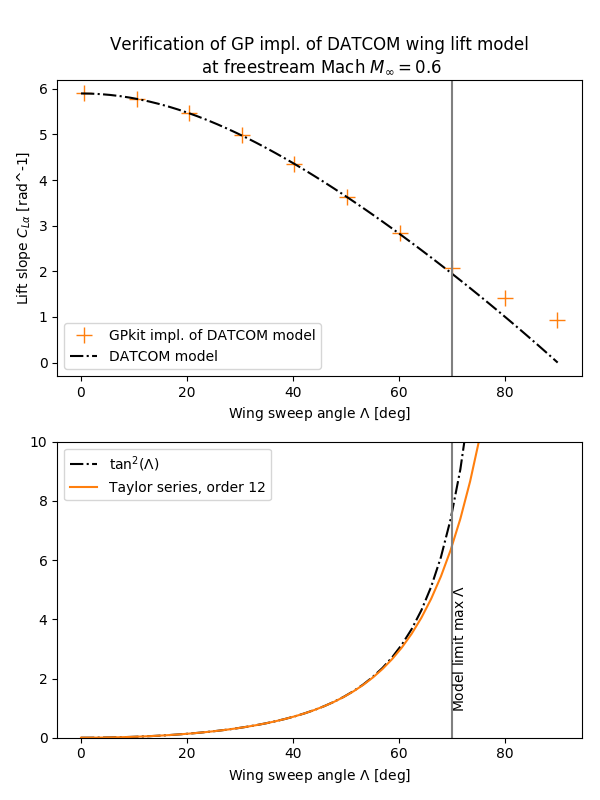
\includegraphics[width=0.8\textwidth]{figures/wing_lift_model_compare/GP_sweep}
    \caption{\label{fig:wing_model_GP_sweep} Comparison of $C_{L\alpha}$ vs. $\Lambda$ predictions for the DATCOM model (as given in \cite{Raymer2012}, black curve) and my GPkit implementation of that model (orange crosses). The GP implementation diverges from the DATCOM model as sweep increases.}
\end{figure}


\subsection{Drag}
We wish to model the drag of a finite, swept wing in compressible flow. 

\subsubsection{Comparison of Models}
\paragraph{DATCOM Model}
I don't think we should use the DATCOM model for drag. It is arcane and looks difficult to implement in GP. Also, DATCOM was compiles in 1978 based on data collected several years earlier. Thus, it may not include advances in transonic/supercritical airfoil design. In fact, the DATCOM model makes no mention of airfoil selection.

A point in favor of the DATCOM model is that uses airfoil $t/c$ as a parameter, which may be useful if we want to explore varying the airfoil thickness for structural reasons. 

\paragraph{Drela's Approach}
Drela \cite{Drela2014} suggests that we tabulate the 2D airfoil performance of the airfoil as a function of Mach number, and then use this data along with lifting line theory to predict the drag of the 3D wing.

Specifically, we parameterize the (2D) performance of the airfoil as $c_{df}(c_l, M_\infty, Re_\infty)$ and $c_{dp}(c_l, M_\infty, Re_\infty)$, the friction and pressure components of drag. These can be computed numerically by \href{http://web.mit.edu/drela/Public/web/mses/}{MSES} and then fit with a GP model via GPfit.

Then, the 3D drag is modeled as:
\begin{equation}
\label{eq:3d_wing_drag_drela}
C_D = c_{df}(M_\infty) + c_{dp}(M_\perp) \cos^3\Lambda + \frac{C_L^2}{\pi \ar e}
\end{equation}

On the right-hand side, the first term is the friction drag at the freestream Mach number. The second term is the pressure drag, which depends on the Mach number \emph{perpendicular to the wing}. In this model, sweep reduces drag by reducing $M_\perp$ for a given $M_\infty$. The third term is the induced drag, and $e$ is the ``span efficiency''. It depends on the aspect ratio $\ar$ and taper $\lambda$ of the wing.

This model is probably only valid for high aspect ratio wings. It assumes that the airflow over the wing is 2D with a spanwise $M_\infty \sin\Lambda$ component superimposed. A low $\ar$ wing may have 3D flow effects that invalidate this assumption.
Also I think the $C_L^2$ induced drag term comes from lifting line theory, which assumes a high aspect ratio wing.
Future work should quantify the minimum aspect ratio at which this model is sufficiently accurate by comparing to  a more sophisticated model (vortex-lattice or volume-discretizing CFD) or wind tunnel data.

There is also some question about the exponent on the $\cos \Lambda$ term multiplying the pressure drag coefficient in Eq. \ref{eq:3d_wing_drag_drela}. Drela \cite{Drela2014} says that this exponent should be $3$, and provides a reasonable theoretical justification. However, Hoerner \cite{Hoerner1965} claims that ``the pressure coefficients reduce in proportion to $\cos \Lambda$'' (i.e. and exponent of $1$).

Figure \ref{fig:wing_model_drag_cos_exp} shows the effect of the cosine exponent on the drag model. Compare this to data on the effect of sweep from other references in Fig. \ref{fig:wing_drag_vs_sweep_refs}. Using $\cos^3$ causes a moderate decrease in drag with increasing sweep at sub-critical Mach numbers. This agrees with Loftin's figure (left of Fig. \ref{fig:wing_drag_vs_sweep_refs}) but not with Hoerner's (right of Fig. \ref{fig:wing_drag_vs_sweep_refs}).

For now I am going to use $\cos^3$, but we should remember that this is an ambiguous choice and revisit it if a) the model does not agree with CFD drag predictions, or b) if the overall model converges to very swept wings for slow-flying aircraft.


\begin{figure}[hbt!]
    \centering
    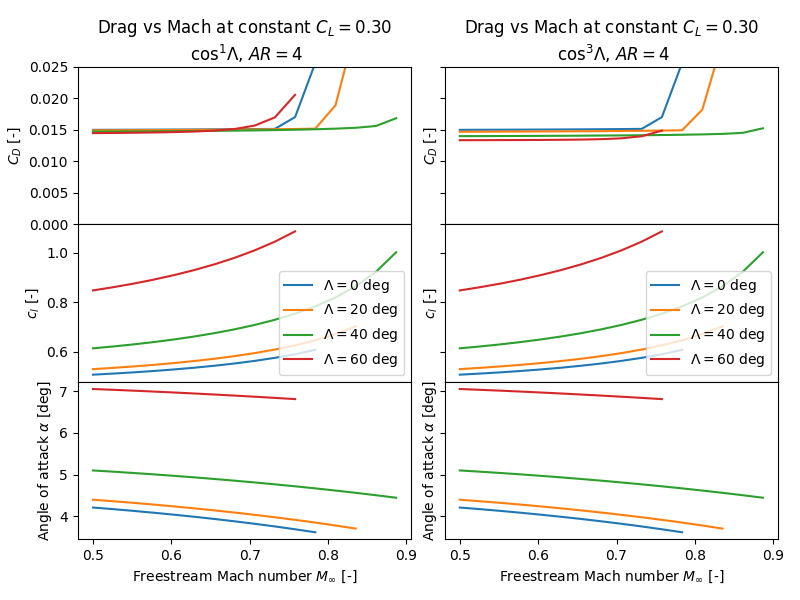
\includegraphics[width=\textwidth]{figures/wing_drag_model/drag_cos_exp}
    \caption{\label{fig:wing_model_drag_cos_exp} Comparison of $C_D$ vs. $M$ predictions for the wing drag model. the left column uses a $\cos\Lambda$ term on the pressure drag, the right column uses $\cos^3 \Lambda$. For sweep angles up to $\Lambda = \SI{40}{\degree}$, increasing sweep (beneficially) pushes the drag divergence to higher Mach numbers. For $\Lambda = \SI{60}{\degree}$, the wing must operate at very high $\alpha$ to achieve $C_L=0.3$, because $C_{L\alpha}$ decreases with sweep. Thus the $\Lambda = \SI{60}{\degree}$ wing reaches the $c_{l, max} = 1.1$ limit of the airfoil model at relatively low Mach number.}
\end{figure}

\begin{figure}[hbt!]
    \centering
    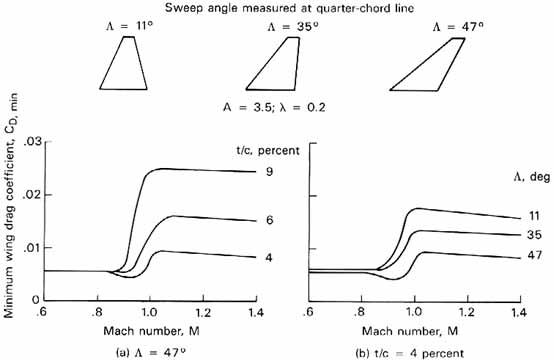
\includegraphics[width=0.45\textwidth]{figures/wing_drag_model/loftin_sweep}
    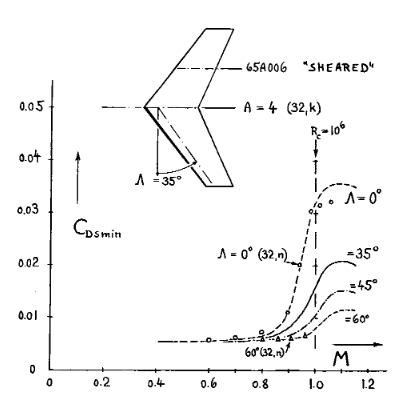
\includegraphics[width=0.45\textwidth]{figures/wing_drag_model/hoerner_fig_15_31}
    \caption{\label{fig:wing_drag_vs_sweep_refs} $C_D$ versus Mach number at various sweep angles, from Loftin \cite{Loftin1985} (right) and Hoerner \cite{Hoerner1965} (left). Compare to our model in the top row of Fig. \ref{fig:wing_model_drag_cos_exp}.}
\end{figure}




We'll need to do some shenanigans to make $\cos$ and $\cos^3$ GP compatible. Their Taylor series about 0 have negative terms.

\printbibliography

\end{document}